
	\section{Our Approach}
	\label{section:app}
    Our entity alignment model can be applied to any two arbitrary (heterogeneous) \KGs. Without loss of generality, we introduce our approach
  using two \KGs: $G_1 = (E_1,V_1,R_1,A_1,T_1)$ and $G_2 = (E_2,V_2,R_2,A_2,T_2)$ for entity alignment, where
$E,V,R,A,T$ represent entities, values, relations, attributes and triples respectively.
	We put $G_1$ and $G_2$ together in one large graph $G$. We utilize pre-aligned entity pairs to train our models and then discover new
equivalent entities. Figure~\ref{all} demonstrates the overall architecture of our model.
	
	
	\begin{figure}[t!]
		\begin{center}
			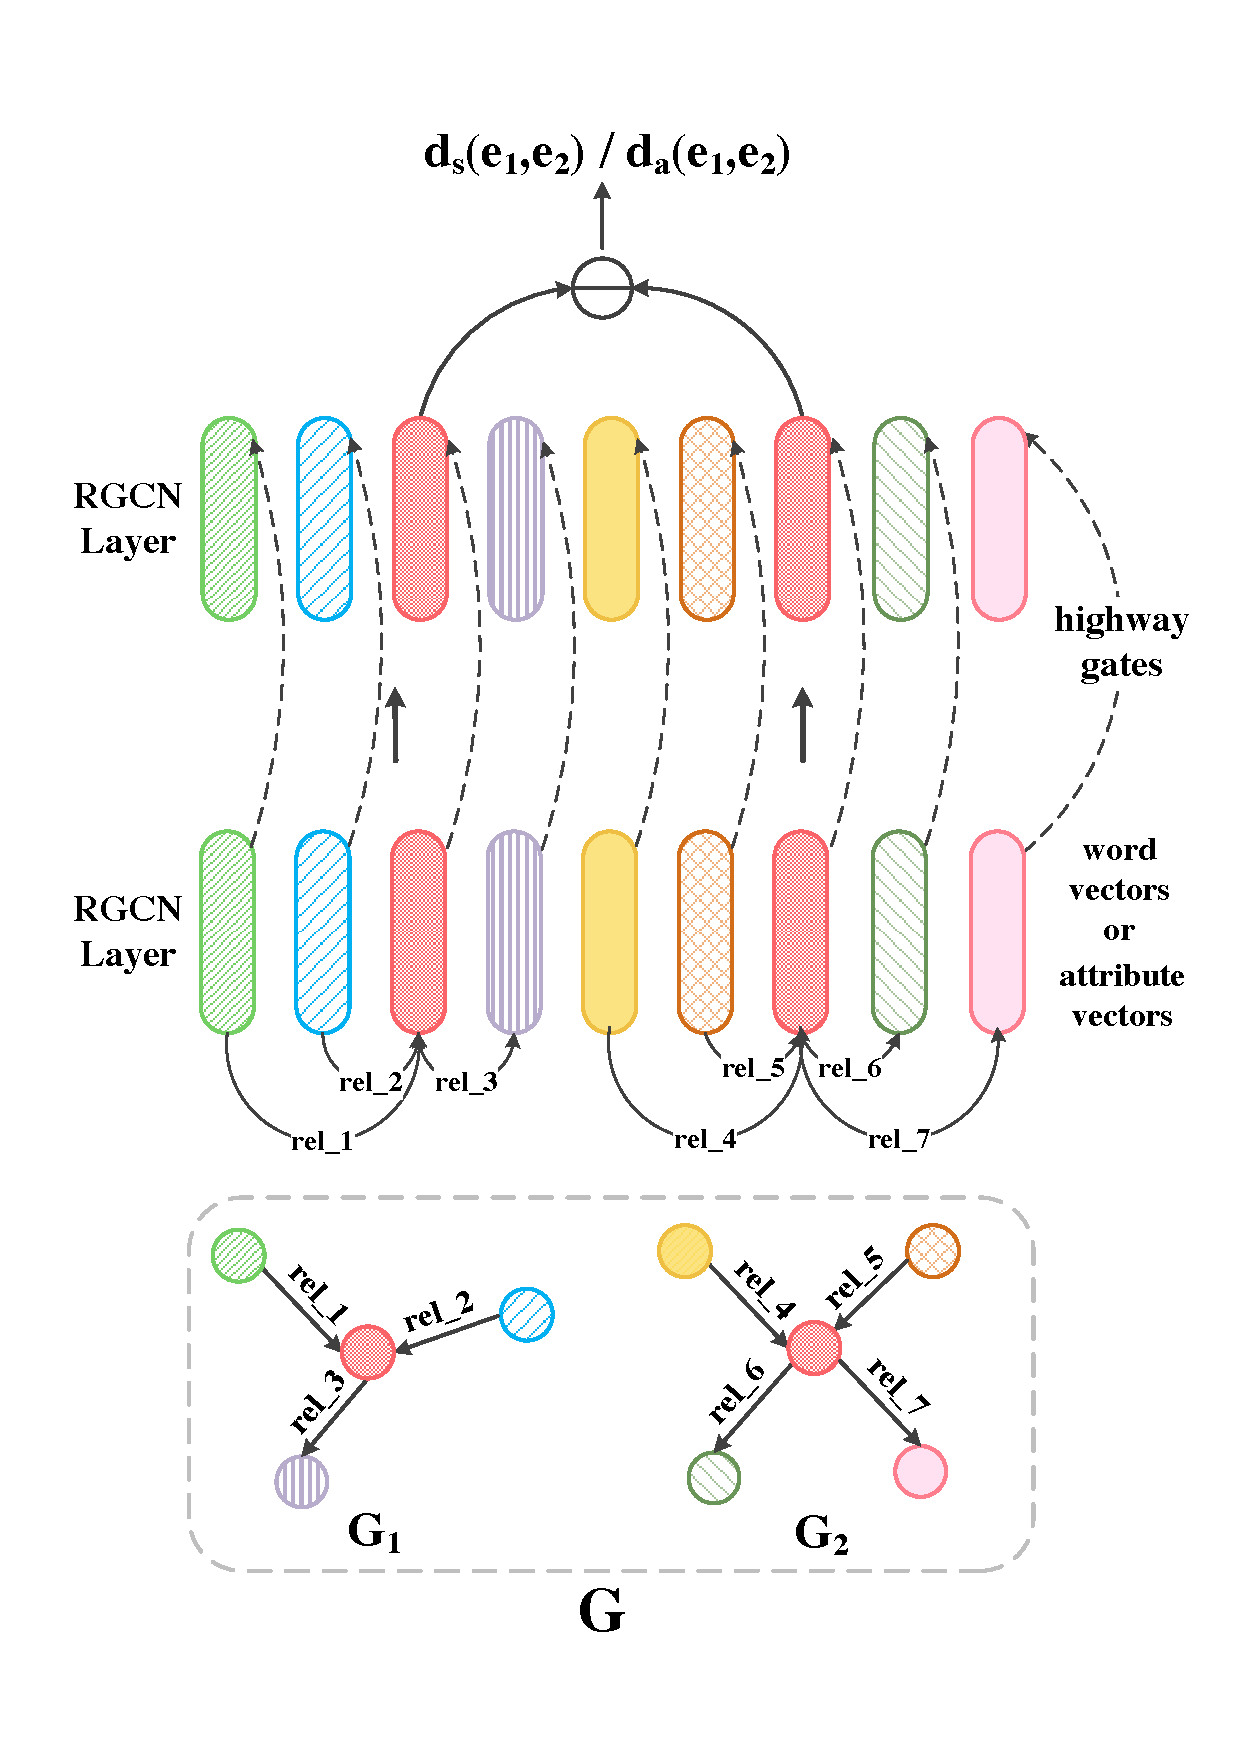
\includegraphics[width=0.8\linewidth]{figures/graph2.pdf}
			\caption{Overall architecture of our entity alignment model.}
			\label{all}
		\end{center}
	\end{figure}
	
    \subsection{Base Model}
    Our approach is based on the recently proposed relational graph convolutional network (\RGCN)~\cite{Schlichtkrull2017Modeling}. A \RGCN takes as
    input \FIXME{XX}, and produces \FIXME{xx}. We choose to use a \RGCN because it can model directed graphs like \KGs. Our work improves the
    featureless approach of \RGCN with pre-defined node feature vectors (\FIXME{Why do you want to do that???}).


	\subsection{Node Representations}
	\label{subsection:Node Representations}
	We combine node semantic information with value information to construct input node feature vectors. The specific construction method is as follows.
    \FIXME{Explain what is node semantic information here...}
	
	\cparagraph{Semantic information}
	\label{wordvector}
	We believe that the entities and their counterparts in multiple \KGs should be semantically similar. Therefore we leverage the pre-trained word embeddings to introduce the semantic information about the surface forms of entities.
	We use word2vec software of Tomas Mikolov and his colleagues\footnote{https://code.google.com/archive/p/word2vec} to generate word embeddings. In our experiments, the window size is 5 and threshold for downsampling the frequent words is 20. Sentences in Baidu baike are used as training data and 155,837 100-dimensional word vectors are generated.
	
	\cparagraph{Value information}
	For attribute values, we distinguish four kinds of abstract range types, i.e., Integer, Double, Date and String (as default). In this paper, we only consider the first three types, i.e., Integer, Double and Date. We overlook String type values by reason of their complexity and heterogeneity in different \KGs.
	
	We construct normalized attribute vector for each entity. Specifically, the dimension of attribute vector is equal to the number of distinct attributes of which the value types belong to Integer, Double and Date in the KG. The elements in an entity’s attribute vector equal to the normalized values of the corresponding attributes. If an entity does not have an attribute, the element corresponding to this attribute in the vector is then set to 0.
	
	We concatenate pre-trained word vectors with attribute vectors as the input feature vectors of entities (nodes) in \KGs.
	
	\subsection{RGCN}
	\label{section:rgcn}
	The input to our RGCN model are two parts. The first part is the node feature matrix $X^{(0)} \in \mathbb{R}^{N \times d^{(0)}}$ of $G$, where $N$ is the number of nodes and $d^{(0)}$ is the dimension of the input representations. We utilize predefined node features described in Section~\ref{subsection:Node Representations} to construct $X$ instead of using a featureless approach in R-GCNs~\cite{Schlichtkrull2017Modeling}.
	The second part is the list of adjacency matrixs $A=\{A_1,A_2,...,A_R |A_i \in \mathbb{R}^{N \times N} \}$, which describes $R$ different relations. We extract $R_0$ original relations from knowledge graphs, then we add reverse relations in order to pass information from the opposite direction; and add the self loop to retain information of the node itself. These together compose $R=2R_0+1$ relations.
	In each layer $l$, the input is $X^{(l-1)} = \{x^{(l-1)}_1,x^{(l-1)}_2,...,x^{(l-1)}_{N} |x^{(l-1)}_{i} \in \mathbb{R}^{d^{(l-1)}}\}$. The forward propagation is formulated as:
	\begin{equation}
	x_i^{(l+1)}=\mathrm{ReLU} (\sum\limits_{r \in R}\sum\limits_{j \in N_i^r} \frac{1}{|N_i^r|}W_r^{(l)}x_j^{(l)})
	\end{equation}
	Here $W_r^{(l)} \in \mathbb{R}^{d^{(l)} \times d^{(l-1)}}$ is the weight matrix of relation $r$. $N_i^r$ is the set of neighbor indices of node $i$ under adjacency matrix $\hat A_r$. $\hat A_r$ is an approximate of spectral convolutions on $A^r$, introduced by ~\cite{Kipf2016Semi}:
	\begin{equation}
	\hat A_r=\hat D_r^{- \frac{1}{2}}(A_r+I)\hat D_r^{- \frac{1}{2}}
	\end{equation}
	where $(\hat D_r)_{jj}=\sum_k(A_r+I)_{jk}$.
	
	We get the new embedding matrix $X^{(l+1)} \in \mathbb{R}^{N \times d^{(l+!)}}$ by stacking the output $x_i^{(l+1)}$ together.
	
	As there are generally thousands of relation types in knowledge graphs, there will be a large amount of parameters to train and the model is likely to overfit. Hence we employ the basis decomposition, which is introduced in ~\cite{Schlichtkrull2017Modeling}, to regularize the weights:
	\begin{equation}
	W_r^{(l)}=\sum\limits_{b=1}^B a_{rb}^{(l)}V_b^{(l)}
	\end{equation}
	where $V_b^{(l)} \in \mathbb{R}^{d^{(l)} \times d^{(l-1)}}$ and $a_{rb}^{(l)}$ is the coefficient of matrix $V_b^{(l)}$ for relation $r$.
	
	
	\subsubsection{Highway RGCN}
	\label{section:hgcn}
	While stacking RGCN layers makes our model capable of learning more neighborhood information from several relational steps, it may as well bring noise from the exponentially increasing neighbors. To reduce the effect of noise and ensure effective spread of more informative and discriminative neighborhood information, we add layer-wise gates similar to highway networks~\cite{Srivastava2015Highway} to our RGCN entity alignment model. ~\cite{Rahimi2018Semi} have successfully introduced highway gates to GCNs~\cite{Kipf2016Semi} to solve the user geolocation problem. We introduce layer-wise highway gates to our RGCN model to finally get Highway RGCN (HRGCN) model and the output of a HRGCN layer is computed as:
	\begin{equation}
	\begin{split}
	&T(x^{(l)})=\sigma(W_T^{(l)}x^{(l)}+b_T^{(l)}) \\
	&x^{(l+1)}=x^{(l+1)} \cdot T(x^{(l)})+x^{(l)} \cdot (1-T(x^{(l)}))
	\end{split}
	\end{equation}
	where $\sigma$ indicates the sigmoid activation function, $\cdot$ is element-wise multiplication, $W_T^{(l)} \in \mathbb{R}^{d^{(l)} \times d^{(l-1)}}$ and $b_T^{(l)} \in \mathbb{R}^{d^{(l)} \times 1}$ are the weight matrix and bias vector of transform gate $T(x^{(l)})$.
	
	\subsection{Alignment Prediction}
	After HRGCN layers, we get the hidden representations $\bar{X}$ of all nodes in both \KGs. We measure the similarity between $e_1$ in $G_1$ and $e_2$ in $G_2$ by the distance between their hidden representations: $d(e_1,e_2)=|\bar{x_{e_1}}-\bar{x_{e_2}}|$, where $|\cdot|$ indicates the $l_1$ norm. The distance for equivalent entities is expected to be smaller than non-equivalent ones. In our experiments, for a entity $e_1$ in $G_1$, we computes the distances between $e_1$ and all the entities in $G_2$.
	
	A set of pre-aligned entity pairs $\mathbb{L}$ and the set of negative pairs $\mathbb{L'}$  constructed by corrupting $(p, q)$, i.e. replacing $p$ or $q$ with a randomly chosen entity in $G_1$ or $G_2$ are used for training. To maximize the distance between positive and negative instances, we use the margin-based loss function:
	\begin{equation}
	L=\sum\limits_{(p,q)\in \mathbb{L}}\sum\limits_{(p',q')\in \mathbb{L'}}\mathrm{max}\{0,d(p_i,q_i)-d(p'_i,q'_i)+\gamma\}
	\end{equation}
	$\gamma > 0$ is a margin hyper-parameter separating positive and negative entity alignments.
	
